\documentclass[tikz,dvisvgm,border=0pt]{standalone}
% Shared preamble of the diagrams in vignettes/articles/cuda-kernels.Rmd.
% Render them with `make diagrams` from the package root.
\usepackage[T1]{fontenc}
\usepackage{lmodern}
\usepackage{tikz}
\usetikzlibrary{arrows.meta, positioning, fit, backgrounds, calc, shapes.geometric, decorations.pathreplacing}

\definecolor{host}{HTML}{3B6EA8}
\definecolor{device}{HTML}{2E8B57}
\definecolor{accent}{HTML}{C0571B}
\definecolor{muted}{HTML}{6B6B6B}

% A white card behind every figure, so that it reads in pkgdown's dark mode.
\tikzset{
  every picture/.append style={
    show background rectangle,
    background rectangle/.style={fill=white, rounded corners=6pt},
    inner frame sep=8pt,
    font=\sffamily\small,
    >={Stealth[length=2.2mm]},
  },
  box/.style={draw, rounded corners=3pt, thick, align=center, inner sep=5pt, fill=white},
  hostbox/.style={box, draw=host, fill=host!8},
  devbox/.style={box, draw=device, fill=device!8},
  accbox/.style={box, draw=accent, fill=accent!8},
  region/.style={draw=#1, rounded corners=6pt, thick, dashed, inner sep=8pt},
  heading/.style={font=\sffamily\bfseries\small, text=#1},
  note/.style={font=\sffamily\footnotesize, text=muted, align=center},
  flow/.style={->, thick},
  code/.style={font=\ttfamily\footnotesize},
}

\begin{document}
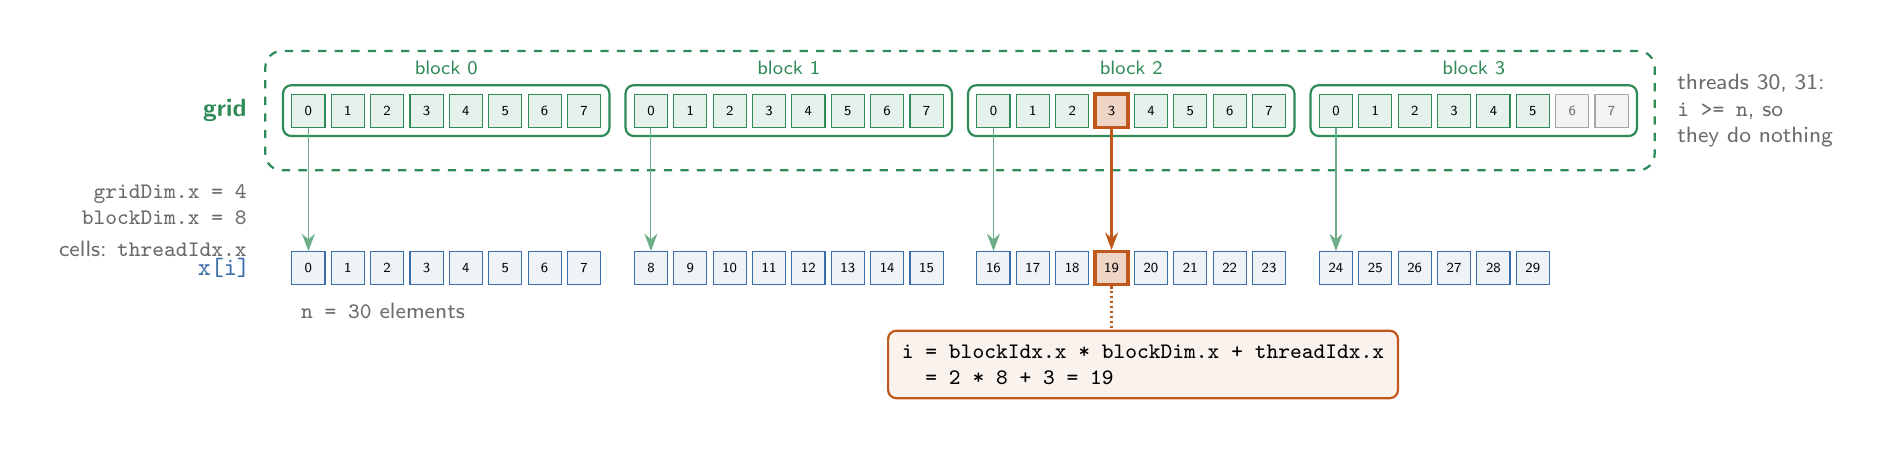
\begin{tikzpicture}[
    thread/.style={draw=device, fill=device!12, minimum size=0.42cm, inner sep=0pt, font=\sffamily\tiny},
    idle/.style={draw=muted!60, fill=muted!8, text=muted, minimum size=0.42cm, inner sep=0pt, font=\sffamily\tiny},
    hit/.style={draw=accent, fill=accent!25, very thick, minimum size=0.42cm, inner sep=0pt, font=\sffamily\tiny},
    elem/.style={draw=host, fill=host!8, minimum width=0.42cm, minimum height=0.42cm, inner sep=0pt, font=\sffamily\tiny},
  ]
  \def\w{0.5}   % pitch of one thread
  \def\gap{0.35} % gap between blocks
  % the grid: 4 blocks of 8 threads
  \foreach \b in {0,...,3} {
    \foreach \t in {0,...,7} {
      \pgfmathtruncatemacro{\i}{8*\b + \t}
      \pgfmathsetmacro{\x}{\b*(8*\w + \gap) + \t*\w}
      \ifnum\i=19
        \node[hit] (t\i) at (\x, 0) {\t};
      \else\ifnum\i>29
        \node[idle] (t\i) at (\x, 0) {\t};
      \else
        \node[thread] (t\i) at (\x, 0) {\t};
      \fi\fi
    }
    \pgfmathtruncatemacro{\first}{8*\b}
    \pgfmathtruncatemacro{\last}{8*\b + 7}
    \node[draw=device, rounded corners=3pt, thick, fit=(t\first)(t\last), inner sep=3pt] (blk\b) {};
    \node[font=\sffamily\scriptsize, text=device, above=0pt of blk\b] {block \b};
  }
  \node[region=device, fit=(blk0)(blk3), inner ysep=12pt, inner xsep=6pt] (grid) {};
  \node[heading=device, anchor=east] at ($(grid.west) + (-0.1, 0)$) {grid};
  \node[note, anchor=north east, align=right] at ($(grid.south west) + (-0.1, -0.05)$)
    {\texttt{gridDim.x = 4}\\\texttt{blockDim.x = 8}\\[2pt]cells: \texttt{threadIdx.x}};

  % the array, one element per thread
  \foreach \i in {0,...,29} {
    \pgfmathtruncatemacro{\b}{int(\i/8)}
    \pgfmathsetmacro{\x}{\b*(8*\w + \gap) + mod(\i,8)*\w}
    \ifnum\i=19
      \node[elem, draw=accent, fill=accent!25, very thick] (e\i) at (\x, -2.0) {\i};
    \else
      \node[elem] (e\i) at (\x, -2.0) {\i};
    \fi
  }
  \node[heading=host, anchor=east] at ($(e0.west) + (-0.4, 0)$) {\texttt{x[i]}};
  \node[note, anchor=north west] at ($(e0.south west) + (0, -0.1)$) {\texttt{n = 30} elements};
  \foreach \i in {0, 8, 16, 24} {
    \draw[->, device!70, thin] (t\i.south) -- (e\i.north);
  }
  \draw[->, accent, very thick] (t19.south) -- (e19.north);

  % the computation of one index
  \node[accbox, anchor=north, code, align=left] (formula) at ($(e19.south) + (0.4, -0.55)$)
    {i = blockIdx.x * blockDim.x + threadIdx.x\\\phantom{i} = 2 * 8 + 3 = 19};
  \draw[accent, thick, densely dotted] (e19.south) -- (formula.north -| e19.south);

  % idle threads
  \node[note, anchor=west, align=left] at ($(grid.east) + (0.15, 0)$)
    {threads 30, 31:\\\texttt{i >= n}, so\\they do nothing};
\end{tikzpicture}
\end{document}
